\documentclass[laporan.tex]{subfiles}

\begin{document}

\chapter{HASIL DAN PEMBAHASAN}

Data berupa foto jeruk yang telah diambil sesuai dengan langkah-langkah yang dijelaskan pada subbab \ref{photoshoot}. Pada penelitian ini dipersiapkan 12 foto dari 6 jeruk. Tabel \ref{table:orangeallstars} menampilkan seluruh foto jeruk yang digunakan dalam penelitian. Setiap jeruk difoto dua kali untuk mendapatkan foto bagian depan dan belakang.

\begin{table}[h!]
\centering
\begin{tabular}{|c|c|c|c|}
\hline
DSC\_2994.JPG & DSC\_2995.JPG & DSC\_2996.JPG & DSC\_2997.JPG \\ 
\includegraphics[width=3.2cm]{DSC_2994.JPG} &
\includegraphics[width=3.2cm]{DSC_2995.JPG} &
\includegraphics[width=3.2cm]{DSC_2996.JPG} &
\includegraphics[width=3.2cm]{DSC_2997.JPG} \\
1a & 1b & 2a & 2b \\
\hline
DSC\_2998.JPG & DSC\_2999.JPG & DSC\_3000.JPG & DSC\_3001.JPG \\ 
\includegraphics[width=3.2cm]{DSC_2998.JPG} &
\includegraphics[width=3.2cm]{DSC_2999.JPG} &
\includegraphics[width=3.2cm]{DSC_3000.JPG} &
\includegraphics[width=3.2cm]{DSC_3001.JPG} \\
3a & 3b & 4a & 4b \\
\hline
DSC\_3002.JPG & DSC\_3003.JPG & DSC\_3004.JPG & DSC\_3005.JPG \\ 
\includegraphics[width=3.2cm]{DSC_3002.JPG} &
\includegraphics[width=3.2cm]{DSC_3003.JPG} &
\includegraphics[width=3.2cm]{DSC_3004.JPG} &
\includegraphics[width=3.2cm]{DSC_3005.JPG} \\
5a & 5b & 6a & 6b \\
\hline
\end{tabular}
\caption{Foto-foto jeruk yang digunakan dalam penelitian}
\label{table:orangeallstars}
\end{table}

Pada bab ini digunakan salah satu foto jeruk sebagai contoh hasil pengolahan data yaitu foto 2a.

\begin{figure}[h]
\centering
\includegraphics[width=8cm]{DSC_2996.JPG}
\caption{Foto jeruk yang diolah}
\end{figure}

\section{Pengolahan Data Awal}

Foto jeruk diperkecil resolusinya dan disunting secara manual untuk menghilangkan objek latar belakang. Hasil akhir pengolahan awal ditunjukkan pada gambar \ref{fig:imgedited}.


\begin{figure}[h!]
\centering
\includegraphics[width=8cm]{DSC_2996.png}
\caption{Gambar yang sudah dibersihkan}
\label{fig:imgedited}
\end{figure}

\section{Pengolahan Dengan Algoritma}

\subsection{\emph{Thresholding}}

\emph{Thresholding} dengan metode Otsu diterapkan pada tiap komponen warna. Nilai \emph{threshold} untuk data contoh ditampilkan di tabel \ref{table:threshval}.

\begin{table}[h]
\centering
\begin{tabular}{|l|l|}
\hline
Komponen warna & Nilai \emph{Threshold} \\
\hline
R & 82 \\
G & 79 \\
B & 44 \\
\hline
\end{tabular}
\caption{Nilai \emph{threshold} metode Otsu}
\label{table:threshval}
\end{table}

\begin{figure}[h!]
\centering
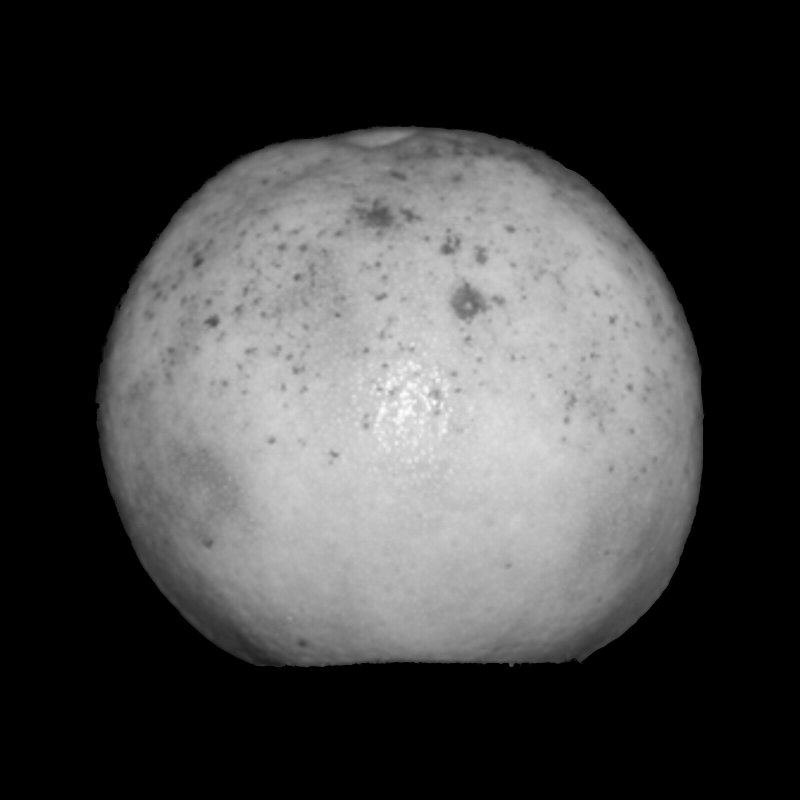
\includegraphics[width=3.2cm]{2996r.png} \hskip 0.5cm
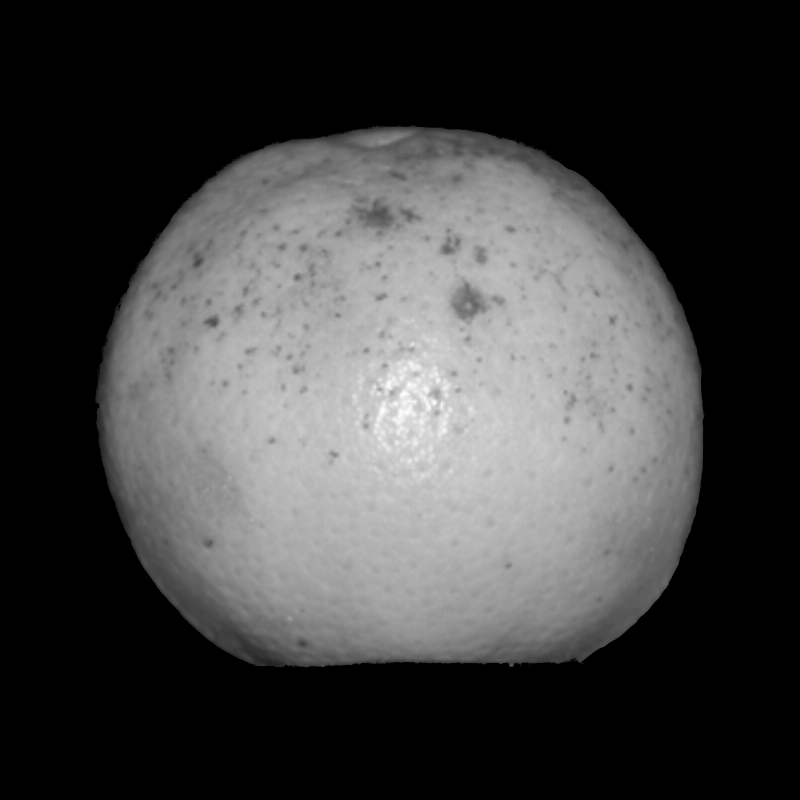
\includegraphics[width=3.2cm]{2996g.png} \hskip 0.5cm
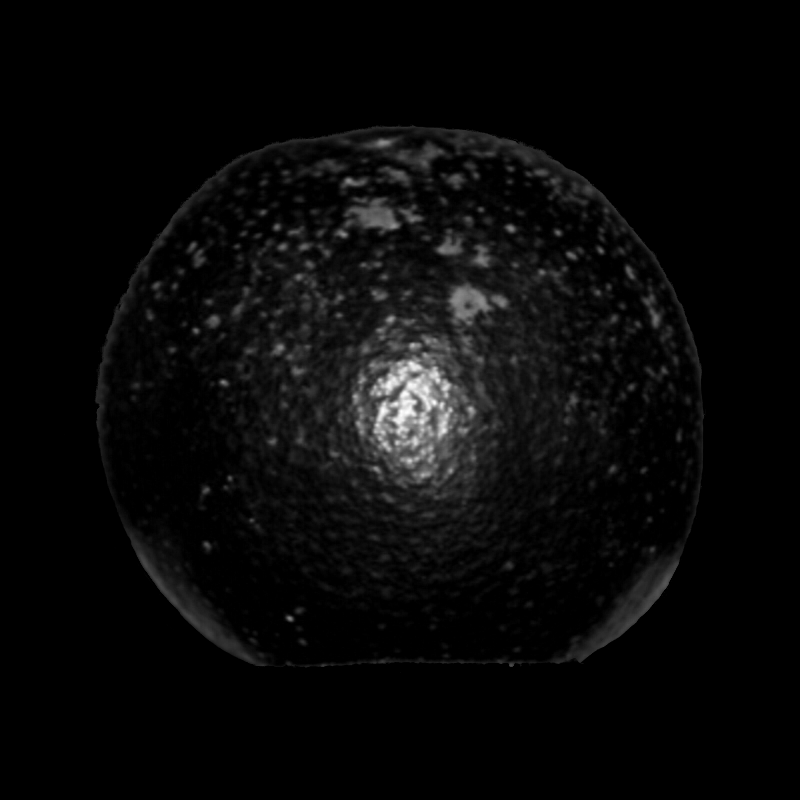
\includegraphics[width=3.2cm]{2996b.png}
\vskip 1cm
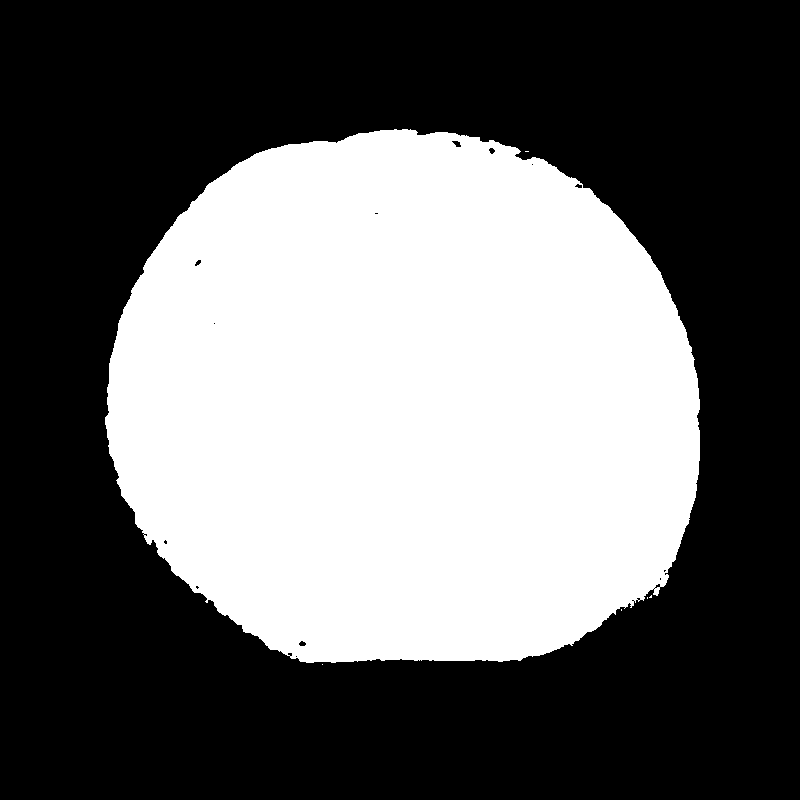
\includegraphics[width=3.2cm]{2996rt.png} \hskip 0.5cm
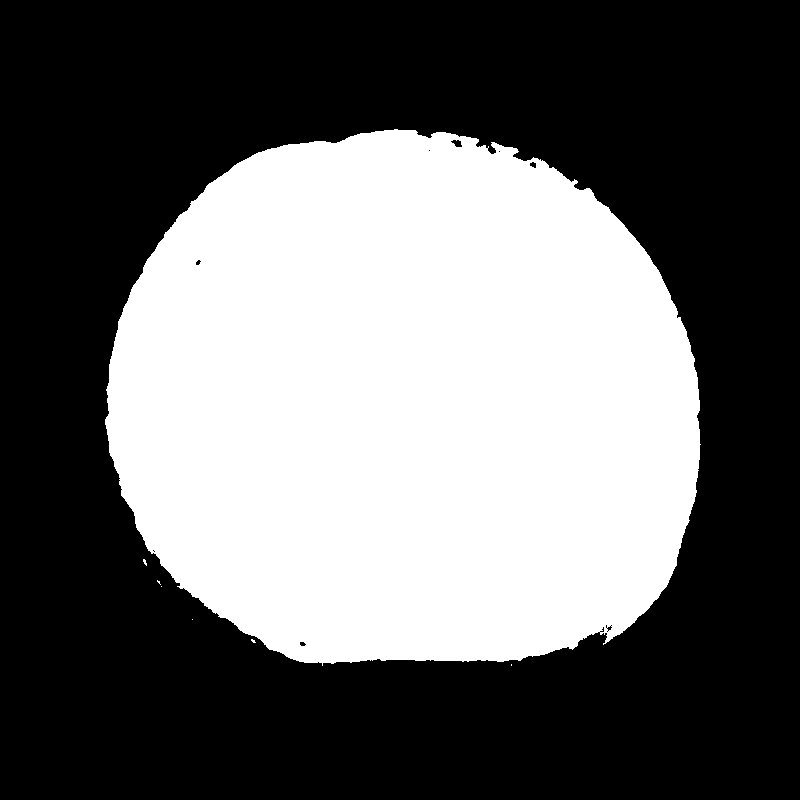
\includegraphics[width=3.2cm]{2996gt.png} \hskip 0.5cm
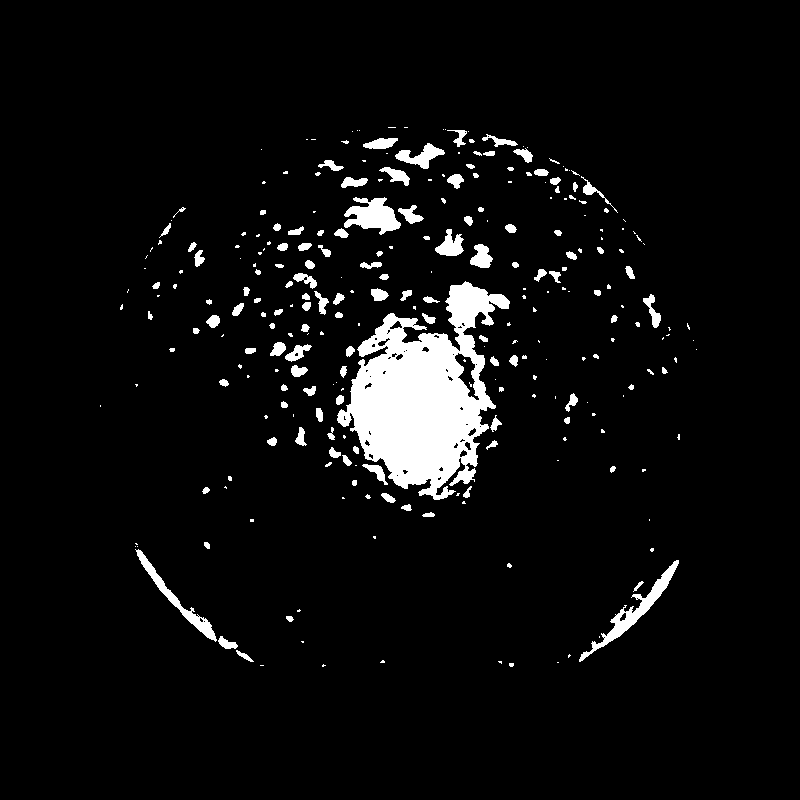
\includegraphics[width=3.2cm]{2996bt.png}
\caption{Hasil operasi \emph{thresholding} pada komponen warna citra R, G, dan B}
\end{figure}

Operasi \emph{threshold} menghasilkan tiga citra biner untuk masing-masing komponen warna. Klasifikasi dapat dilakukan ke \emph{pixel} data citra dengan menerapkan langsung \mbox{rumus} \ref{classcol} pada ketiga citra biner sehingga dihasilkan matriks integer yang menyimpan nilai kelas untuk data \emph{pixel} citra.

Hasil operasi \emph{thresholding} menunjukkan bahwa komponen warna biru pada citra jeruk mempunyai intensitas yang rendah, sebaliknya komponen warna merah dan hijau mempunyai intensitas lebih tinggi dan tersebar merata pada hampir seluruh permukaan jeruk yang tampak. Hal ini dapat dipahami sebagai akibat dari karakteristik warna jeruk yang didominasi oleh warna hijau dan kuning. Komponen warna biru justru mempunyai intensitas lebih tinggi pada daerah-daerah yang secara visual tampak sebagai bagian cacat dari kulit jeruk.

\subsection{Klasifikasi \emph{Pixel} Awal}

Klasifikasi awal dilakukan dengan \emph{weighted sum} dari ketiga citra biner hasil \emph{thresholding} untuk ketiga komponen warna. \emph{Pixel} citra jeruk diklasifikasikan berdasarkan keberadaan komponen warna primer. Hasil klasifikasi adalah matriks integer dengan rentang nilai $[1..8]$. Dari matriks ini dihitung banyaknya \emph{pixel} yang dimasukkan ke masing-masing kelas sehingga dapat diketahui rata-rata intensitas tiga komponen warna dari masing-masing kelas.

Hasil klasifikasi awal membagi jeruk menjadi 8 kelas berdasarkan segmentasi komponen-komponen warna primer dengan metode Otsu. Pada contoh ditunjukkan visualisasi hasil klasifikasi pada gambar \ref{fig:classinit}, nilai-nilai intensitas asli \emph{pixel} digantikan dengan rata-rata intensitas kelas masing-masing \emph{pixel} tersebut. Tabel rata-rata intensitas tabel \ref{table:clsrgbavg1} menunjukkan bahwa seluruh kelas warna muncul pada citra yang diuji.

\begin{figure}[h]
\centering
\includegraphics[width=8cm]{seg3a.png}
\caption{Visualisasi hasil klasifikasi \emph{pixel} awal}
\label{fig:classinit}
\end{figure}

\begin{table}[h]
\centering
\begin{tabular}{|l|l|l|l|}
\cline{1-4}
\multirow{2}{*}{Kelas} & \multicolumn{3}{l|}{Rata-rata intensitas} \\
\cline{2-4}
 & R & G & B \\
\cline{1-4}
1 & 1.67 & 0.72 & 0.75 \\
2 & 61.11 & 68.35 & 51.13 \\
3 & 76.11 & 82.57 & 21.15 \\
4 & 73.85 & 87.14 & 57.80 \\
5 & 84.01 & 76.80 & 25.06 \\
6 & 82.90 & 77.18 & 49.90 \\
7 & 160.50 & 154.17 & 11.82 \\
8 & 180.61 & 177.75 & 85.59 \\
\cline{1-4}
\end{tabular}
\caption{Nilai rata-rata intensitas tiap kelas}
\label{table:clsrgbavg1}
\end{table}

\subsubsection{Pembuatan Kelas Baru}

Kelas-kelas \emph{pixel} selanjutnya disusun ulang berdasarkan jarak antarkelas yang dihitung dari \emph{mean squared distance} rata-rata intensitas. Kelas yang saling bertetangga digabungkan kemudian rata-rata intensitas baru dihitung untuk tiap kelas. Tabel \ref{table:clsdist} menunjukkan hasil perhitungan jarak antarkelas untuk data contoh, tabel \ref{table:newclass} menunjukkan kelas baru yang dibuat. Tabel \ref{table:newclassavg} memuat rata-rata intensitas kelas baru.


\begin{table}[h]
\centering
\begin{tabular}{|l|l|l|l|l|l|l|l|l|}
\hline
Kelas & K1 & K2 & K3 & K4 & K5 & K6 & K7 & K8 \\
\hline
K1 & -- & 59.20 & 64.79 & 72.49 & 65.85 & 70.03 & 127.27 & 153.05 \\
K2 & 59.20 & -- & 21.18 & 13.66 & 20.62 & 13.60 & 79.14 & 95.68 \\
K3 & 64.79 & 21.18 & --	& 21.39 & 5.80 & 17.26 & 63.84 & 89.52 \\
K4 & 72.49 & 13.66 & 21.39 & --	& 20.67 & 9.01 & 68.59 & 82.46 \\
K5 & 65.85 & 20.62 & 5.80 & 20.67 & -- & 14.36 & 63.28 & 88.00 \\
K6 & 70.03 & 13.60 & 17.26 & 9.01 & 14.36 & -- & 66.83 & 83.59 \\
K7 & 127.27 & 79.14 & 63.84 & 68.59 & 63.28 & 66.83 & -- & 46.39 \\
K8 & 153.05 & 95.68 & 89.52 & 82.46 & 88.00 & 83.59 & 46.39 & -- \\
\hline
\end{tabular}
\caption{Jarak antarkelas}
\label{table:clsdist}
\end{table}

\begin{table}[h]
\centering
\begin{tabular}{|l|l|l|}
\hline
Kelas & Kelas Terdekat & Kelas Baru \\
\hline
K1 & K2 & K1 \\
K2 & K6 & K2 \\
K3 & K5 & K3 = K3 + K5 \\
K4 & K6 & K4 = K4 + K6 \\
K5 & K3 & -- \\
K6 & K4 & -- \\
K7 & K8 & K5 = K7 + K8 \\
K8 & K7 & -- \\
\hline
\end{tabular}
\caption{Penggabungan kelas}
\label{table:newclass}
\end{table}

\begin{table}[h]
\centering
\begin{tabular}{|l|l|l|l|}
\cline{1-4}
\multirow{2}{*}{Kelas} & \multicolumn{3}{l|}{Rata-rata intensitas} \\
\cline{2-4}
 & R & G & B \\
\cline{1-4}
1 & 1.67 & 1.72 & 0.75 \\
2 & 61.11 & 68.35 & 51.13 \\
3 & 78.62 & 81.10 & 22.14 \\
4 & 74.50 & 86.43 & 57.24 \\
5 & 163.00 & 157.10 & 21.04 \\
\cline{1-4}
\end{tabular}
\caption{Rata-rata intensitas kelas baru}
\label{table:newclassavg}
\end{table}

\subsubsection{Reklasifikasi \emph{Pixel}}

\emph{Pixel} pada citra asli diklasifikasi ulang berdasarkan jarak terdekat dari nilai rata-rata intensitas dengan perhitungan \emph{sum squared distance}. Gambar \ref{fig:classfinimg} menunjukkan hasil klasifikasi ulang, nilai intensitas asli tiap \emph{pixel} diganti dengan rata-rata intensitas kelas untuk memvisualisasikan matriks kelas \emph{pixel}.

\begin{figure}[h]
\centering
\includegraphics[width=8cm]{seg3b.png}
\caption{Hasil klasifikasi ulang \emph{pixel}}
\label{fig:classfinimg}
\end{figure}

\subsection{Operasi Morfologi}

Dari matriks data klasifikasi akhir dilakukan \emph{thresholding} untuk mengambil titik-titik \emph{pixel} dengan kelas yang mempunyai rata-rata intensitas tertinggi sebagai sebuah citra biner yang menunjukkan bagian teksur normal. Operasi morfologi penutupan lubang dilakukan atas citra biner ini lalu diambil selisihnya untuk mendeteksi bagian-bagian cacat.

\begin{figure}[h!]
\centering
\includegraphics[width=4cm]{seg3b.png} \qquad
\includegraphics[width=4cm]{mask3normal.png}
\caption{Operasi \emph{thresholding} pada matriks klasifikasi akhir dan citra biner yang dihasilkan}
\label{fig:finclassthresh}
\end{figure}

Gambar \ref{fig:finclassthresh} menunjukkan bahwa bagian tepi masuk ke dalam kelas dengan intensitas yang lebih rendah. Hal ini disebabkan oleh penyinaran yang diterima bagian tepi tidak sebanyak bagian tengah karena perbedaan sudut datang sinar yang mengenai bagian tersebut. Sementara itu di bagian tengah dapat dilihat bahwa variasi warna yang cukup mencolok pada daerah normal tidak mempengaruhi hasil klasifikasi sehingga perbedaan warna di daerah normal tidak menimbulkan kesalahan deteksi daerah cacat, sebagaimana ditunjukkan oleh gambar \ref{fig:greenyellow}.%161 393 166 166

\begin{figure}[h!]
\centering
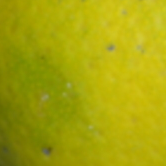
\includegraphics[width=2.5cm]{cropgreen1.png} \qquad

\includegraphics[width=2.5cm]{cropgreen2.png}
\caption{Pengaruh variasi warna pada deteksi}
\label{fig:greenyellow}
\end{figure}

\begin{figure}[h!]
\centering
\includegraphics[width=4cm]{mask3normal.png} \qquad
\includegraphics[width=4cm]{mask3filled.png} \qquad
\includegraphics[width=4cm]{mask3blemish.png}
\caption{\emph{Mask} tekstur normal, hasil penutupan lubang dan cacat yang dideteksi}
\end{figure}

Tabel \ref{table:pixelcountexample} adalah data-data jumlah \emph{pixel} yang didapatkan pada gambar di atas.

\begin{table}[h!]
\centering
\begin{tabular}{|l|l|}
\hline
Data & Jumlah \emph{pixel} \\
\hline
Daerah normal & 221386 \\
Daerah cacat & 3615 \\
\hline
\end{tabular}
\caption{Data perhitungan jumlah \emph{pixel}}
\label{table:pixelcountexample}
\end{table}

\section{Perhitungan Luas Cacat dan Akurasi}

Sebagai acuan akurasi deteksi, digunakan citra biner cacat tekstur kulit yang digambar secara manual dengan menggunakan perangkat \emph{fuzzy select} dan \emph{color select} pada aplikasi pengolah citra Gimp. Luas daerah yang dapat diproses dibandingkan dengan dengan keseluruhan luas objek jeruk dalam citra untuk memperoleh prosentase luas deteksi.

\begin{figure}[h!]
\centering
\includegraphics[width=4cm]{mask3blemish.png} \qquad
\includegraphics[width=4cm]{manDSC_2996.png}
\caption{Hasil deteksi dengan pemrosesan dan hasil penandaan manual}
\end{figure}

\begin{figure}[h!]
\centering
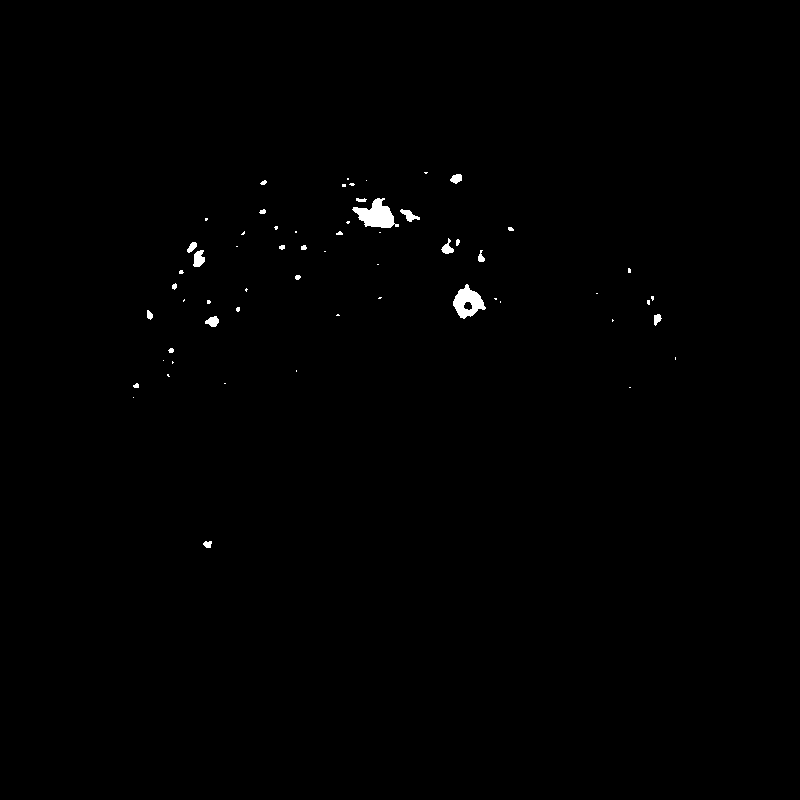
\includegraphics[width=4cm]{tp3.png} \qquad
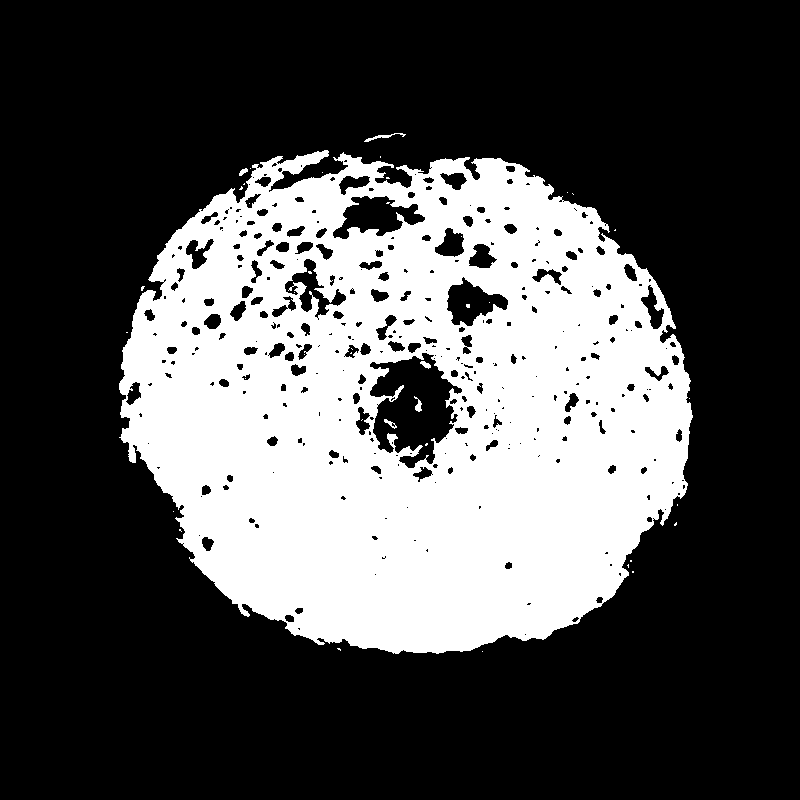
\includegraphics[width=4cm]{tn3.png} \vskip 0.5cm
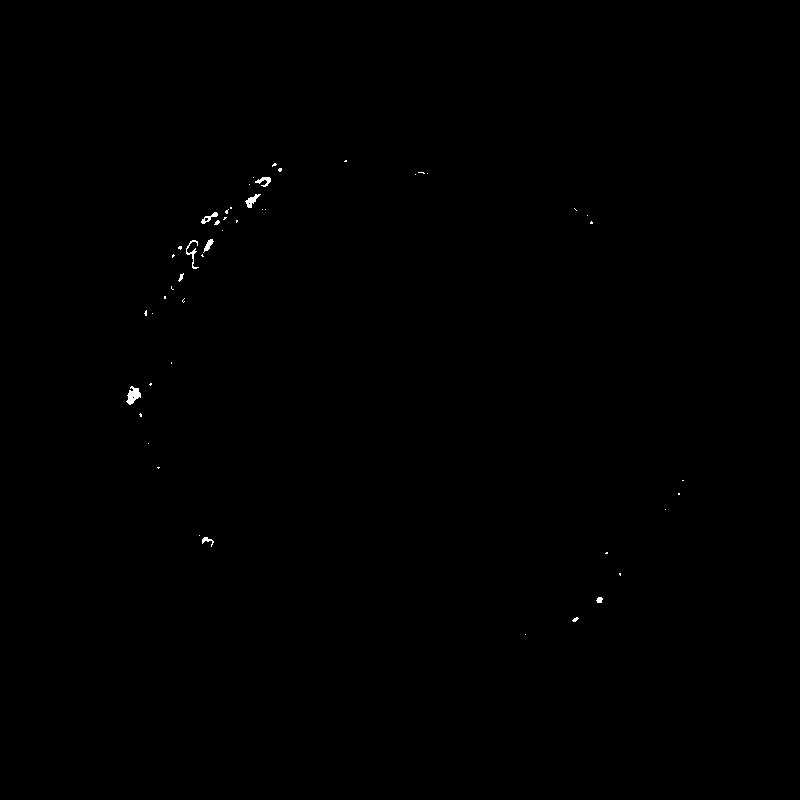
\includegraphics[width=4cm]{fp3.png} \qquad
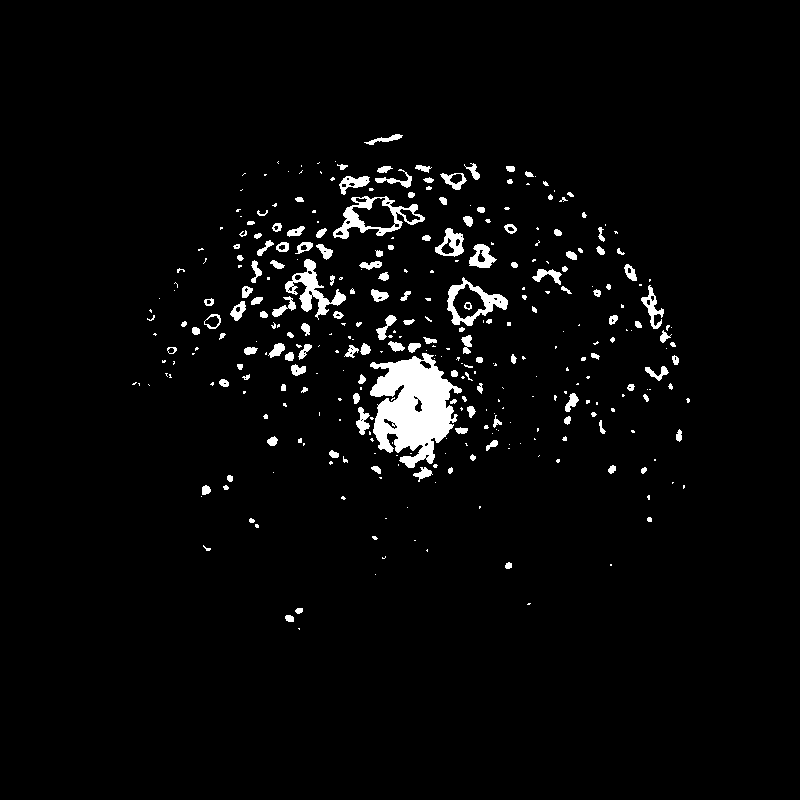
\includegraphics[width=4cm]{fn3.png}
\caption{\emph{Mask} pengujian hasil deteksi: \emph{true positive}, \emph{true negative}, \emph{false positive}, \emph{false negative}}
\end{figure}

\begin{figure}[h!]
\centering
\includegraphics[width=4cm]{mask3filled.png} \qquad

\includegraphics[width=4cm]{detected3.png}
\caption{Perbandingan bagian jeruk yang dapat dideteksi dengan keseluruhan permukaan jeruk pada citra}
\end{figure}

\begin{table}[h!]
\centering
\begin{tabular}{|l|l|}
\hline
Data & Jumlah \emph{pixel} \\
\hline
$TP$ & 2731 \\
$FP$ & 884 \\
$TN$ & 200468 \\
$FN$ & 20918 \\
Area deteksi & 225001 \\
Total area objek & 271992 \\
\hline
\end{tabular}
\caption{Tabel perhitungan akurasi deteksi}
\label{table:confuse3}
\end{table}

Dari data Tabel \ref{table:confuse3} didapatkan ukuran presisi, akurasi dan \emph{recall} untuk pemrosesan data sampel.

\begin{align*}
presisi & = \frac{2731}{2731 + 884}  = 0.76 \\
akurasi & = \frac{2731+200468}{2731+200468+884+20918}  = 0.90 \\
recall & = \frac{2731}{2731+20918}  = 0.12
\end{align*}

Prosentase permukaan yang dapat dideteksi.

\begin{equation*}
deteksi =\frac{221386}{271992} \ast 100\% = 82.72\%
\end{equation*}

Prosentase hasil deteksi dan akurasi dari semua data eksperimen ditunjukkan pada tabel \ref{table:detrecap}.

\begin{table}[h!]
\centering
\begin{tabular}{|l|l|l|l|l|}
\hline
Data & $n$ \emph{pixel} normal & $n$ \emph{pixel} \emph{hole fill} & $n$ \emph{pixel} cacat & \% cacat \\
\hline
1a & 241788&243449&1661&0.682\\
1b & 37995&38716&721&1.862\\
2a & 221386&225001&3615&1.607\\
2b & 229222&230548&1326&0.575\\
3a & 175995&182726&6731&3.684\\
3b & 121087&130677&9590&7.339\\
4a & 163142&169382&6240&3.684\\
4b & 173986&176931&2945&1.664\\
5a & 181115&184190&3075&1.669\\
5b & 171486&173386&1900&1.096 \\
6a & 163276&166109&2833&1.706 \\
6b & 184366&186877&2511&1.344 \\
\hline
\end{tabular}
\caption{Hasil deteksi \emph{pixel} daerah cacat}
\label{table:detrecap}
\end{table}

Perbandingan akurasi dengan hasil penandaan manual ditunjukkan pada tabel \ref{table:detconfuse}.

\begin{table}[h!]
\tiny
\centering
%\resizebox{0.9\textwidth
\begin{tabular} {|l|l|l|l|l|l|l|l|l|l|l|}
\hline
Data & $n$ total & $n$ det.&  $TP$ & $FP$ & $TN$ & $FN$ & \% Presisi & \% Akurasi & \% \emph{Recall} & \% deteksi \\
\hline
1a & 300646&243449&503&1158&234702&64283&30.283&78.233&0.776&80.975 \\
1b & 288910&38716&4&717&217481&70708&0.555&75.278&0.006&13.401 \\
2a & 271992&225001&2731&884&231064&37313&75.546&85.957&6.820&82.723 \\
2b & 271792&230548&1027&299&235938&34528&77.451&87.186&2.888&84.825 \\
3a & 254135&182726&628&6103&152056&95348&9.330&60.080&0.654&71.901 \\
3b & 252699&130677&6151&3439&86852&156257&64.140&36.804&3.787&51.713 \\
4a & 241675&169382&5924&316&129974&105461&94.936&56.232&5.318&70.087 \\
4b & 242394&176931&2378&567&148804&90645&80.747&62.370&2.556&72.993 \\
5a & 262047&184190&2081&994&142149&116823&67.675&55.040&1.750&70.289 \\
5b & 256038&173386&523&1377&130057&124081&27.526&51.000&0.420&67.719 \\
6a & 257723&166109&2542&291&157311&97579&89.728&62.025&2.539&64.453 \\
6b & 255593&186877&1816&695&173834&79248&72.322&68.723&2.240&73.115 \\
\hline
\end{tabular}
\normalsize
\caption{Akurasi dan luas deteksi hasil pemrosesan}
\label{table:detconfuse}
\end{table}

\begin{table}[h!]
\centering
\begin{tabular}{|c|c|c|c|c|}
\hline
& Foto & Normal & Cacat & Det. Manual \\
\hline
1a &
\includegraphics[width=3cm]{DSC_2994.png} &
\includegraphics[width=3cm]{mask1normal.png} &
\includegraphics[width=3cm]{mask1blemish.png} &
\includegraphics[width=3cm]{manDSC_2994.png} \\
\hline
1b &
\includegraphics[width=3cm]{DSC_2995.png} &
\includegraphics[width=3cm]{mask2normal.png} &
\includegraphics[width=3cm]{mask2blemish.png} &
\includegraphics[width=3cm]{manDSC_2995.png} \\
\hline
2a &
\includegraphics[width=3cm]{DSC_2997.png} &
\includegraphics[width=3cm]{mask3normal.png} &
\includegraphics[width=3cm]{mask3blemish.png} &
\includegraphics[width=3cm]{manDSC_2997.png} \\
\hline
2b &
\includegraphics[width=3cm]{DSC_2996.png} &
\includegraphics[width=3cm]{mask4normal.png} &
\includegraphics[width=3cm]{mask4blemish.png} &
\includegraphics[width=3cm]{manDSC_2996.png} \\
\hline
3a &
\includegraphics[width=3cm]{DSC_2998.png} &
\includegraphics[width=3cm]{mask5normal.png} &
\includegraphics[width=3cm]{mask5blemish.png} &
\includegraphics[width=3cm]{manDSC_2998.png} \\
\hline
3b &
\includegraphics[width=3cm]{DSC_2999.png} &
\includegraphics[width=3cm]{mask6normal.png} &
\includegraphics[width=3cm]{mask6blemish.png} &
\includegraphics[width=3cm]{manDSC_2999.png} \\
\hline
\end{tabular}
\caption{Hasil deteksi cacat dengan pemrosesan dan penandaan manual (bagian 1)}
\label{table:fodderpls}
\end{table}

\begin{table}[h!]
\centering
\itshape{(Lanjutan)}
\begin{tabular}{|c|c|c|c|c|}
\hline
& Foto & Normal & Cacat & Det. Manual \\
4a &
\includegraphics[width=3cm]{DSC_3000.png} &
\includegraphics[width=3cm]{mask7normal.png} &
\includegraphics[width=3cm]{mask7blemish.png} &
\includegraphics[width=3cm]{manDSC_3000.png} \\
\hline
4b &
\includegraphics[width=3cm]{DSC_3001.png} &
\includegraphics[width=3cm]{mask8normal.png} &
\includegraphics[width=3cm]{mask8blemish.png} &
\includegraphics[width=3cm]{manDSC_3001.png} \\
\hline
5a &
\includegraphics[width=3cm]{DSC_3002.png} &
\includegraphics[width=3cm]{mask9normal.png} &
\includegraphics[width=3cm]{mask9blemish.png} &
\includegraphics[width=3cm]{manDSC_3002.png} \\
\hline
5b &
\includegraphics[width=3cm]{DSC_3003.png} &
\includegraphics[width=3cm]{mask10normal.png} &
\includegraphics[width=3cm]{mask10blemish.png} &
\includegraphics[width=3cm]{manDSC_3003.png} \\
\hline
6a &
\includegraphics[width=3cm]{DSC_3004.png} &
\includegraphics[width=3cm]{mask11normal.png} &
\includegraphics[width=3cm]{mask11blemish.png} &
\includegraphics[width=3cm]{manDSC_3004.png} \\
\hline
6b &
\includegraphics[width=3cm]{DSC_3005.png} &
\includegraphics[width=3cm]{mask12normal.png} &
\includegraphics[width=3cm]{mask12blemish.png} &
\includegraphics[width=3cm]{manDSC_3005.png} \\
\hline
\end{tabular}
\caption{Hasil deteksi cacat dengan pemrosesan dan penandaan manual (bagian 2)}
\label{table:fodderpls2}
\end{table}


\FloatBarrier
\section{Perbandingan Hasil}

Untuk perbandingan hasil akan dipilih beberapa data yang memiliki ciri signifikan.

\begin{enumerate}
\item Jeruk dengan warna dominan kuning: data 2a
\item Jeruk dengan warna dominan hijau: data 4a
\item Jeruk dengan hasil \emph{recall} yang rendah: data 1b
\end{enumerate}

\subsection{Data Jeruk Kuning}

\begin{figure}[h!]
\centering
\includegraphics[width=4cm]{DSC_2996.png}
\includegraphics[width=4cm]{seg3a.png}
\caption[]{Hasil klasifikasi awal data 2a}
\end{figure}

\begin{table}[h!]
\centering
\begin{tabular}{|l|l|l|l|}
\cline{1-4}
\multirow{2}{*}{Kelas} & \multicolumn{3}{l|}{Rata-rata intensitas} \\
\cline{2-4}
 & R & G & B \\
\cline{1-4}
1 & 1.67 & 0.72 & 0.75 \\
2 & 61.11 & 68.35 & 51.13 \\
3 & 76.11 & 82.57 & 21.15 \\
4 & 73.85 & 87.14 & 57.80 \\
5 & 84.01 & 76.80 & 25.06 \\
6 & 82.90 & 77.18 & 49.90 \\
7 & 160.50 & 154.17 & 11.82 \\
8 & 180.61 & 177.75 & 85.59 \\
\cline{1-4}
\end{tabular}
\caption[]{Nilai rata-rata intensitas tiap kelas data 2a}
\label{table:avgyellow1}
\end{table}

\begin{table}[h!]
\centering
\begin{tabular}{|l|l|l|l|l|l|l|l|l|}
\hline
Kelas & K1 & K2 & K3 & K4 & K5 & K6 & K7 & K8 \\
\hline
K1 & -- & 59.20 & 64.79 & 72.49 & 65.85 & 70.03 & 127.27 & 153.05 \\
K2 & 59.20 & -- & 21.18 & 13.66 & 20.62 & 13.60 & 79.14 & 95.68 \\
K3 & 64.79 & 21.18 & --	& 21.39 & 5.80 & 17.26 & 63.84 & 89.52 \\
K4 & 72.49 & 13.66 & 21.39 & --	& 20.67 & 9.01 & 68.59 & 82.46 \\
K5 & 65.85 & 20.62 & 5.80 & 20.67 & -- & 14.36 & 63.28 & 88.00 \\
K6 & 70.03 & 13.60 & 17.26 & 9.01 & 14.36 & -- & 66.83 & 83.59 \\
K7 & 127.27 & 79.14 & 63.84 & 68.59 & 63.28 & 66.83 & -- & 46.39 \\
K8 & 153.05 & 95.68 & 89.52 & 82.46 & 88.00 & 83.59 & 46.39 & -- \\
\hline
\end{tabular}
\caption[]{Jarak antarkelas data 2a}
\label{table:distyellow}
\end{table}

\begin{table}[h!]
\centering
\begin{tabular}{|l|l|l|}
\hline
Kelas & Kelas Terdekat & Kelas Baru \\
\hline
K1 & K2 & K1 \\
K2 & K6 & K2 \\
K3 & K5 & K3 = K3 + K5 \\
K4 & K6 & K4 = K4 + K6 \\
K5 & K3 & -- \\
K6 & K4 & -- \\
K7 & K8 & K5 = K7 + K8 \\
K8 & K7 & -- \\
\hline
\end{tabular}
\caption[]{Kelas baru data 2a}
\label{table:clsyellow2}
\end{table}

\begin{figure}[h!]
\centering
\includegraphics[width=4cm]{seg3b.png}
\caption[]{Hasil klasifikasi akhir data 2a}
\end{figure}

\begin{figure}[h!]
\centering
\includegraphics[width=4cm]{mask3normal.png} \qquad
\includegraphics[width=4cm]{mask3blemish.png}
\caption[]{Hasil deteksi daerah normal dan cacat 2a}
\end{figure}

\begin{table}[h!]
\centering
\begin{tabular}{|l|l|l|l|}
\cline{1-4}
\multirow{2}{*}{Kelas} & \multicolumn{3}{l|}{Rata-rata intensitas} \\
\cline{2-4}
 & R & G & B \\
\cline{1-4}
1 & 1.67 & 1.72 & 0.75 \\
2 & 61.11 & 68.35 & 51.13 \\
3 & 78.62 & 81.10 & 22.14 \\
4 & 74.50 & 86.43 & 57.24 \\
5 & 163.00 & 157.10 & 21.04 \\
\cline{1-4}
\end{tabular}
\caption[]{Rata-rata intensitas kelas baru data 2a}
\label{table:avgyellow2}
\end{table}

Data menunjukkan variasi intensitas yang relatif rendah dengan kontras antara daerah normal dan daerah cacat tinggi. Cakupan daerah yang terproses luas karena intensitas tinggi yang merata meliputi sebagian besar permukaan jeruk. Kontras yang tinggi antara daerah cacat dan daerah normal menyebabkan akurasi deteksi relatif tinggi di antara data lainnya.

%\clearpage
\FloatBarrier
\subsection{Data Jeruk Hijau}

\begin{figure}[h!]
\centering
\includegraphics[width=4cm]{DSC_3000.png}
\includegraphics[width=4cm]{seg7a.png}
\caption[]{Hasil klasifikasi awal data 4a}
\end{figure}

Jeruk hijau mempunyai variasi warna yang lebih banyak daripada jeruk kuning. Daerah intensitas tinggi yang dapat dideteksi sedikit lebih sempit daripada jeruk kuning, akurasinya sebanding dengan data jeruk kuning. Dari contoh data terlihat bahwa cacat di bagian tengah tidak terdeteksi karena adanya kilap dari pantulan cahaya.

\begin{table}[h]
\centering
\begin{tabular}{|l|l|l|l|}
\cline{1-4}
\multirow{2}{*}{Kelas} & \multicolumn{3}{l|}{Rata-rata intensitas} \\
\cline{2-4}
 & R & G & B \\
\cline{1-4}
1 & 1.27 & 1.46 & 0.79 \\
2 & 48.50 & 53.72 & 48.35 \\
3 & 55.43 & 67.73 & 17.54 \\
4 & 55.84 & 65.47 & 53.39 \\
5 & 60.80 & 61.27 & 27.77 \\
6 & 60.81 & 61.49 & 60.69 \\
7 & 111.68 & 120.88 & 19.96 \\
8 & 121.95 & 128.78 & 77.75 \\
\cline{1-4}
\end{tabular}
\caption[]{Nilai rata-rata intensitas tiap kelas data 4a}
\label{table:avggreen1}
\end{table}

\begin{table}[h]
\centering
\begin{tabular}{|l|l|l|l|l|l|l|l|l|}
\hline
Kelas & K1 & K2 & K3 & K4 & K5 & K6 & K7 & K8 \\
\hline
K1 & -- & 49.07 & 50.35 & 57.28 & 51.15 & 59.82 & 94.55 & 110.60 \\
K2 & 49.07 & -- & 19.95 & 8.51 & 14.51 & 11.02 & 55.70 & 62.96 \\
K3 & 50.35 & 19.95 & -- & 20.74 & 7.64 & 25.36 & 44.70 & 62.65 \\
K4 & 57.28 & 8.51 & 20.74 & -- & 15.26 & 5.59 & 49.35 & 54.68 \\
K5 & 51.15 & 14.51 & 7.64 & 15.26 & -- & 19.00 & 45.47 & 59.98 \\
K6 & 59.82 & 11.02 & 25.36 & 5.59 & 19.00 & -- & 50.90 & 53.41 \\
K7 & 94.55 & 55.70 & 44.70 & 49.35 & 45.47 & 50.90 & -- & 34.19 \\
K8 & 110.60 & 62.96 & 62.65 & 54.68 & 59.98 & 53.41 & 34.19 & -- \\
\hline
\end{tabular}
\caption[]{Jarak antarkelas data 4a}
\label{table:distgreen}
\end{table}

\begin{table}[h]
\centering
\begin{tabular}{|l|l|l|}
\hline
Kelas & Kelas Terdekat & Kelas Baru \\
\hline
K1 & K2 & K1 \\
K2 & K4 & K2 \\
K3 & K5 & K3 = K3 + K5 \\
K4 & K6 & K4 = K4 + K6 \\
K5 & K3 & -- \\
K6 & K4 & -- \\
K7 & K8 & K5 = K7 + K8 \\
K8 & K7 & -- \\
\hline
\end{tabular}
\caption[]{Kelas baru data 4a}
\label{table:clsgreen2}
\end{table}

\begin{figure}[h]
\centering
\includegraphics[width=4cm]{seg7b.png}
\caption[]{Hasil klasifikasi akhir data 4a}
\end{figure}

\begin{figure}[h]
\centering
\includegraphics[width=4cm]{mask7normal.png} \qquad
\includegraphics[width=4cm]{mask7blemish.png}
\caption[]{Hasil deteksi daerah normal dan cacat 4a}
\end{figure}

\begin{table}[h!]
\centering
\begin{tabular}{|l|l|l|l|}
\cline{1-4}
\multirow{2}{*}{Kelas} & \multicolumn{3}{l|}{Rata-rata intensitas} \\
\cline{2-4}
 & R & G & B \\
\cline{1-4}
1 & 1.27 & 1.46 & 0.79 \\
2 & 48.50 & 53.72 & 48.35 \\
3 & 55.51 & 67.63 & 17.70 \\
4 & 57.18 & 64.40 & 55.36 \\
5 & 117.30 & 125.20 & 51.60 \\
\cline{1-4}
\end{tabular}
\caption[]{Rata-rata intensitas kelas baru data 4a}
\label{table:avggreen2}
\end{table}

\FloatBarrier
\subsection{Data Dengan Tingkat \emph{Recall} Rendah}

Data 1b merupakan data dengan tingkat \emph{recall} yang sangat rendah.

\begin{figure}[h!]
\centering
\includegraphics[width=4cm]{DSC_2995.png}
\includegraphics[width=4cm]{seg2a.png}
\caption[]{Hasil klasifikasi awal data 1b}
\end{figure}

\begin{table}[h!]
\centering
\begin{tabular}{|l|l|l|l|}
\cline{1-4}
\multirow{2}{*}{Kelas} & \multicolumn{3}{l|}{Rata-rata intensitas} \\
\cline{2-4}
 & R & G & B \\
\cline{1-4}
1 & 4.61 & 5.46 & 2.99 \\
2 & 60.00 & 62.50 & 68.00 \\
3 & 57.65 & 72.09 & 18.70 \\
4 & 60.00 & 72.00 & 68.00 \\
5 & 64.14 & 65.23 & 27.44 \\
6 & 64.83 & 64.83 & 69.33 \\
7 & 112.24 & 125.97 & 19.24 \\
8 & 152.74 & 172.17 & 126.82 \\
\cline{1-4}
\end{tabular}
\caption[]{Nilai rata-rata intensitas tiap kelas data 1b}
%\label[]{table:avglow1}
\end{table}

\begin{table}[h!]
\centering
\begin{tabular}{|l|l|l|l|l|l|l|l|l|}
\hline
Kelas & K1 & K2 & K3 & K4 & K5 & K6 & K7 & K8 \\
\hline
K1 & -- & 59.29 & 50.00 & 62.51 & 50.71 & 62.06 & 93.75 & 147.27 \\
K2 & 59.29 & -- & 29.03 & 5.48 & 23.59 & 3.19 & 55.18 & 89.61 \\
K3 & 50.00 & 29.03 & -- & 28.49 & 7.43 & 29.82 & 44.28 & 101.24 \\
K4 & 62.51 & 5.48 & 28.49 & -- & 23.86 & 5.05 & 51.70 & 85.82 \\
K5 & 50.71 & 23.59 & 7.43 & 23.86 & -- & 24.19 & 44.98 & 98.59 \\
K6 & 62.06 & 3.19 & 29.82 & 5.05 & 24.19 & -- & 53.21 & 86.70 \\
K7 & 93.75 & 55.18 & 44.28 & 51.70 & 44.98 & 53.21 & -- & 71.53 \\
K8 & 147.27 & 89.61 & 101.24 & 85.82 & 98.59 & 86.70 & 71.53 & -- \\
\hline
\end{tabular}
\caption[]{Jarak antarkelas data 1b}
\label{table:distlow}
\end{table}

\begin{table}[h!]
\centering
\begin{tabular}{|l|l|l|}
\hline
Kelas & Kelas Terdekat & Kelas Baru \\
\hline
K1 & K3 & K1 = K1 + K3 \\
K2 & K6 & K2 \\
K3 & K1 & K1 = K1 + K3 \\
K4 & K6 & K4 = K4 + K6 \\
K5 & K3 & K5 \\
K6 & K2 & -- \\
K7 & K8 & K6 = K7 + K8 \\
K8 & K7 & -- \\
\hline
\end{tabular}
\caption[]{Kelas baru data 1b}
%\label{table:clslow2}
\end{table}


\begin{figure}[h!]
\centering
\includegraphics[width=4cm]{seg2b.png}
\caption[]{Hasil klasifikasi akhir data 1b}
\end{figure}

\begin{figure}[h!]
\centering
\includegraphics[width=4cm]{mask2normal.png} \qquad
\includegraphics[width=4cm]{mask2blemish.png}
\caption[]{Hasil deteksi daerah normal dan cacat 1b}
\end{figure}

\begin{table}[h!]
\centering
\begin{tabular}{|l|l|l|l|}
\cline{1-4}
\multirow{2}{*}{Kelas} & \multicolumn{3}{l|}{Rata-rata intensitas} \\
\cline{2-4}
 & R & G & B \\
\cline{1-4}
1 & 4.61 & 5.46 & 2.99 \\
2 & 63.63 & 64.25 & 69.00 \\
3 & 58.15 & 71.56 & 19.38 \\
4 & 60.00 & 72.00 & 68.00 \\
5 & 112.24 & 125.97 & 19.24 \\
6 & 152.74 & 172.17 & 126.82 \\
\cline{1-4}
\end{tabular}
\caption[]{Rata-rata intensitas kelas baru data 1b}
%\label{table:avglow}
\end{table}

Data citra jeruk 1b memperlihatkan adanya kilap di tengah objek. Perbedaan intensitas kilap ini cukup tinggi dibandingkan dengan daerah lain sehingga membentuk kelas tersendiri yang sebagian besar terdiri dari \emph{pixel-pixel} di daerah kilap. Akibatnya, bagian selain kilap tidak masuk area deteksi. Hanya 13\% dari keseluruhan luas objek jeruk di dalam citra yang terproses, sedangkan pemrosesan tidak dapat bekerja dengan akurat untuk bagian yang berkilap.

\FloatBarrier

\section{Interpretasi Hasil}

Data menunjukkan bahwa metode deteksi menghasilkan hasil yang bervariasi, dengan akurasi tinggi, presisi yang cukup baik, namun \emph{recall} sangat rendah. Tingkat \emph{recall} yang rendah ini disebabkan karena hanya sebagian dari permukaan jeruk yang dapat dideteksi, dan terutama karena citra biner yang digunakan untuk referensi kurang akurat.

Metode ini selain tidak dirancang untuk mendeteksi cacat pada bagian-bagian gelap pada tepi jeruk, juga tidak dapat mendeteksi cacat pada bagian tengah jeruk yang berkilap karena sorotan sumber cahaya. Perlu dilakukan penyesuaian pencahayaan untuk mengurangi atau menghindari munculnya kilap di tengah objek.

\end{document}
